%%%%%%%%%%%%%%%%%% ANOTHER LECTURE

\chapter{Kaluza-Klein Reduction}

The Kaluza-Klein program aims to obtain the $d$-dimensional theory obtained by reducing a $D$-dimensional one. The original idea was to obtain four-dimensional gravity and electrodynamics, from five-dimensional gravity... All of it in the context of general relativity.

In the following the dimensional reduction of the action of a scalar field on $D+1$-dimension to $D$-dimensions is shown, and later, the reduction of $D+1$-dimensional gravity on a $S^1$.  A nice reference to the program is  \cite{PopeKK}.

\section{Reduction of a Scalar Field}

On this section the reduction of a massless, real, scalar field is performed on different manifolds. All over the section it is assumed that the total manifold is nothing but a Cartesian product of two other manifolds.



\subsection{Scalar Field Reduced on $S^1$}
\label{sec:KKs:s1}

Consider the equation of motion of a massless (real) scalar field $\Phi$ on $D+1$-dimensions, 
\begin{equation}
  \Box^{(D+1)} \Phi = 0.
\end{equation}
Assume that $M^{D+1} = M^D \times S^1$. Then,  the differential operator can be separated  into a $D$-dimensional part plus the extra dimension,
\begin{equation}
  \( \Box^{(D)} + \pa{\xi}^2 \) \Phi = 0.
  \label{KK-s-eq:s1}
\end{equation}

Now, one propose the Kaluza-Klein ansatz, i.e., the scalar field can be expanded as a series on the basis of eigenfunctions on $S^1$,
\begin{equation}
  \Phi(x,\xi) = \sum_n \phi_n(x) e^{\imath \frac{n}{R}\xi},
  \label{KK-scalar:s1}
\end{equation}
where $R$ is the radius of the extra dimension.

Substituting the expansion in Eq.~\eqref{KK-scalar:s1} into~\eqref{KK-s-eq:s1}, yields
\begin{equation}
  \[ \Box^{(D)} - \( \frac{n}{R} \)^2 \] \phi_n(x) = 0 \qquad \forall \; n \in \Z.
  \label{KK-eq-s1}
\end{equation}

Comparing with the generic Klein-Gordon equation,
\begin{equation}
  \[ \Box^{(D)} - m_{\text{eff}}^2 \] \phi_n = 0, \qquad \text{with} \qquad m_{\text{eff}} = \frac{ \abs{n} }{ R },
  \label{KKs-m:s1}
\end{equation}
one concludes that Eq.~\eqref{KK-eq-s1}  represents  a tower of infinite massive scalar fields in $D$ dimensions; doubly degenerated because of the blindness on the sign of $n$, plus a single massless scalar field, corresponding to $n = 0$.

\begin{center}
  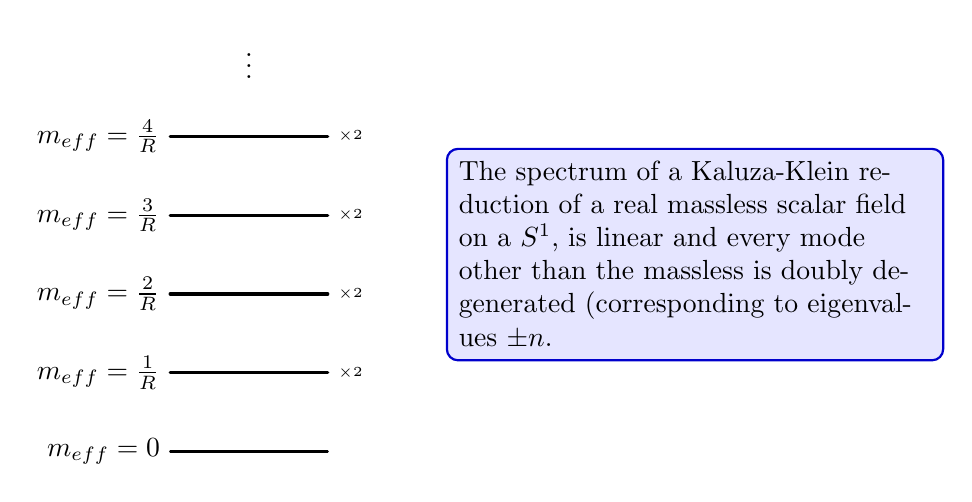
\begin{tikzpicture}[thick,line cap=round,
      % Styles
      axes/.style=,
      important line/.style={very thick},
      information text/.style={rounded corners,draw=blue!80!black,fill=blue!10,inner sep=1ex}]
    
    \draw (0,0) node[anchor=east] {$m_{\text{eff}} =0$} -- (2,0);
    \foreach \y in {1,2,...,4}
    \draw[important line] (0,\y) node[anchor=east] {$m_{\text{eff}} =\frac{\y}{R}$} -- (2,\y);
    \foreach \y in {1,2,...,4}
    \node[anchor=west] at (2,\y) {{\tiny $ \times 2$}};

    \node at (1,5) {$\vdots$};

    \draw[xshift=3.5cm,yshift=2.5cm]
    node[right,text width=6cm,information text]
    {The spectrum of a Kaluza-Klein reduction of a real massless scalar field on a $S^1$, is linear and every mode other than the massless is doubly degenerated (corresponding to eigenvalues $\pm n$.};
  \end{tikzpicture}
\end{center}

\subsection{Scalar Field Reduced on $S^2$}
\label{sec:KKs:s2}

One can follow the previous procedure to compute the \KK of a massless real scalar field on $S^2$. Thus, assuming that $M^{D+2} = M^D \times S^2$, the differential operator separates on,
\begin{equation}
  \( \Box^{(D)} + \Lap \) \Phi = 0.
  \label{KKs-eq:s2}
\end{equation}
Then, the \KK ansatz is done as an expansion on eigenfunctions of the 2-dimensional Laplacian on spherical coordinates, i.e., spherical harmonics, as
\begin{equation}
  \Phi(x,\xi) = \sum_{l,m} \phi_{l,m}(x) \, Y^{lm}(\xi),
\end{equation}
where $Y^{lm}$ satisfy
\begin{equation}
  \Lap Y^{lm} = -\frac{ l(l+1) }{ R^2 } Y^{lm}.
\end{equation}

Therefore, Eq.~\eqref{KKs-eq:s2} yields
\begin{equation}
  \[ \Box^{(D)} - \frac{ l(l+1) }{ R^2 } \] \phi_{l,m}(x) = 0.
  \label{KK-eq-s2}
\end{equation}
Equation~\eqref{KK-eq-s2} represents a \KK tower composed by: a single massless scalar field, corresponding to $l = 0$; and $(2l+1)$-degenerated massive scalar fields with and effective mass
\begin{equation}
  m_{\text{eff}} = \frac{ \sqrt{ l(l+1) } }{ R }.
  \label{KKs-m:s2}
\end{equation}

\begin{center}
  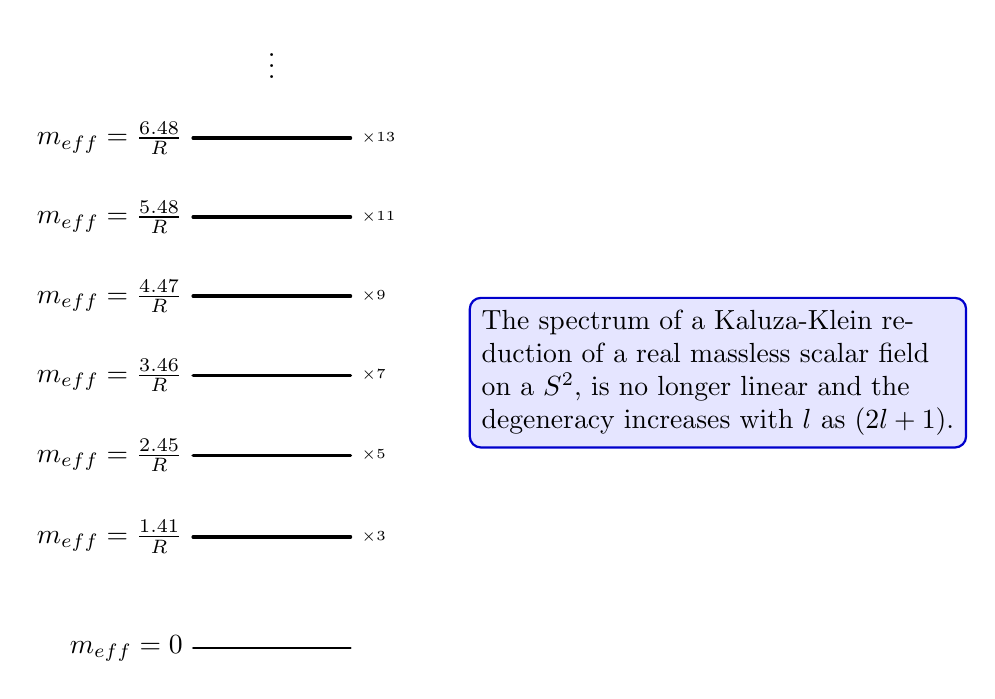
\begin{tikzpicture}[thick,line cap=round,
      % Styles
      axes/.style=,
      important line/.style={very thick},
      information text/.style={rounded corners,draw=blue!80!black,fill=blue!10,inner sep=1ex}]
    \pgfkeys{/pgf/number format/.cd,fixed,precision=2}

    \draw (0,0) node[anchor=east] {$m_{\text{eff}} =0$} -- (2,0);
    \foreach \y/\m in {1/3,2/5,3/7,4/9,5/11,6/13}
             {
               \draw[important line] (0,{sqrt(\y*\y + \y) }) node[anchor=east] {$m_{\text{eff}} =\frac{\pgfmathparse{sqrt(\y*\y + \y) }\pgfmathprintnumber{\pgfmathresult}}{R}$} -- (2,{sqrt(\y*\y + \y) }) node[anchor=west]  {{\tiny $ \times\m$}};
             }
             \node at (1,7.5) {$\vdots$};

             \draw[xshift=3.5cm,yshift=3.5cm]
             node[right,text width=6cm,information text]
             {The spectrum of a Kaluza-Klein reduction of a real massless scalar field on a $S^2$, is no longer linear and the degeneracy increases with $l$ as $(2l+1)$.};
  \end{tikzpicture}
\end{center}

\subsection{Scalar Field Reduced on $T^2$}
\label{sec:KKs:t2}

Once more, inspired in the previous procedure, and using the fact that $T^2 = S^1 \times S^1$, the differential operator separates on,
\begin{equation}
  \( \Box^{(D)} + \pa{\xi_1}^2 + \pa{\xi_2}^2 \) \Phi = 0,
  \label{KKs-eq:t2}
\end{equation}
and the \KK ansatz is
\begin{equation}
  \Phi(x, \xi) = \sum_{m,n} \phi_{m,n}(x) \, e^{\imath \( \frac{m}{R_1} \xi_1 + \frac{n}{R_2} \xi_2 \)},
  \label{KK-scalar:t2}
\end{equation}
where $R_1$ and $R_2$ are the radii of the torus.

Substituting the expansion in Eq.~\eqref{KK-scalar:t2} into~\eqref{KKs-eq:t2}, yields
\begin{equation}
  \[ \Box^{(D)} - \( \frac{m}{R_1} \)^2 - \( \frac{n}{R_2} \)^2 \] \phi_{m,n}(x)= 0 \qquad \forall \; m, n \in \Z.
  \label{KK-eq-t2}
\end{equation}

Equation~\eqref{KK-eq-t2} represents a tower of \KK modes which contains a massless singlet, and infinite massive modes whose degeneracy depend on the relation between the integers $m,n$ and the radii $R_1$ and $R_2$. The effective mass for the \KK modes is
\begin{equation}
  m_{\text{eff}} =  \sqrt{\(\frac{m}{R_1}\)^2+\(\frac{n}{R_2}\)^2}.\label{KKs-m:t2}
\end{equation}

\begin{center}
  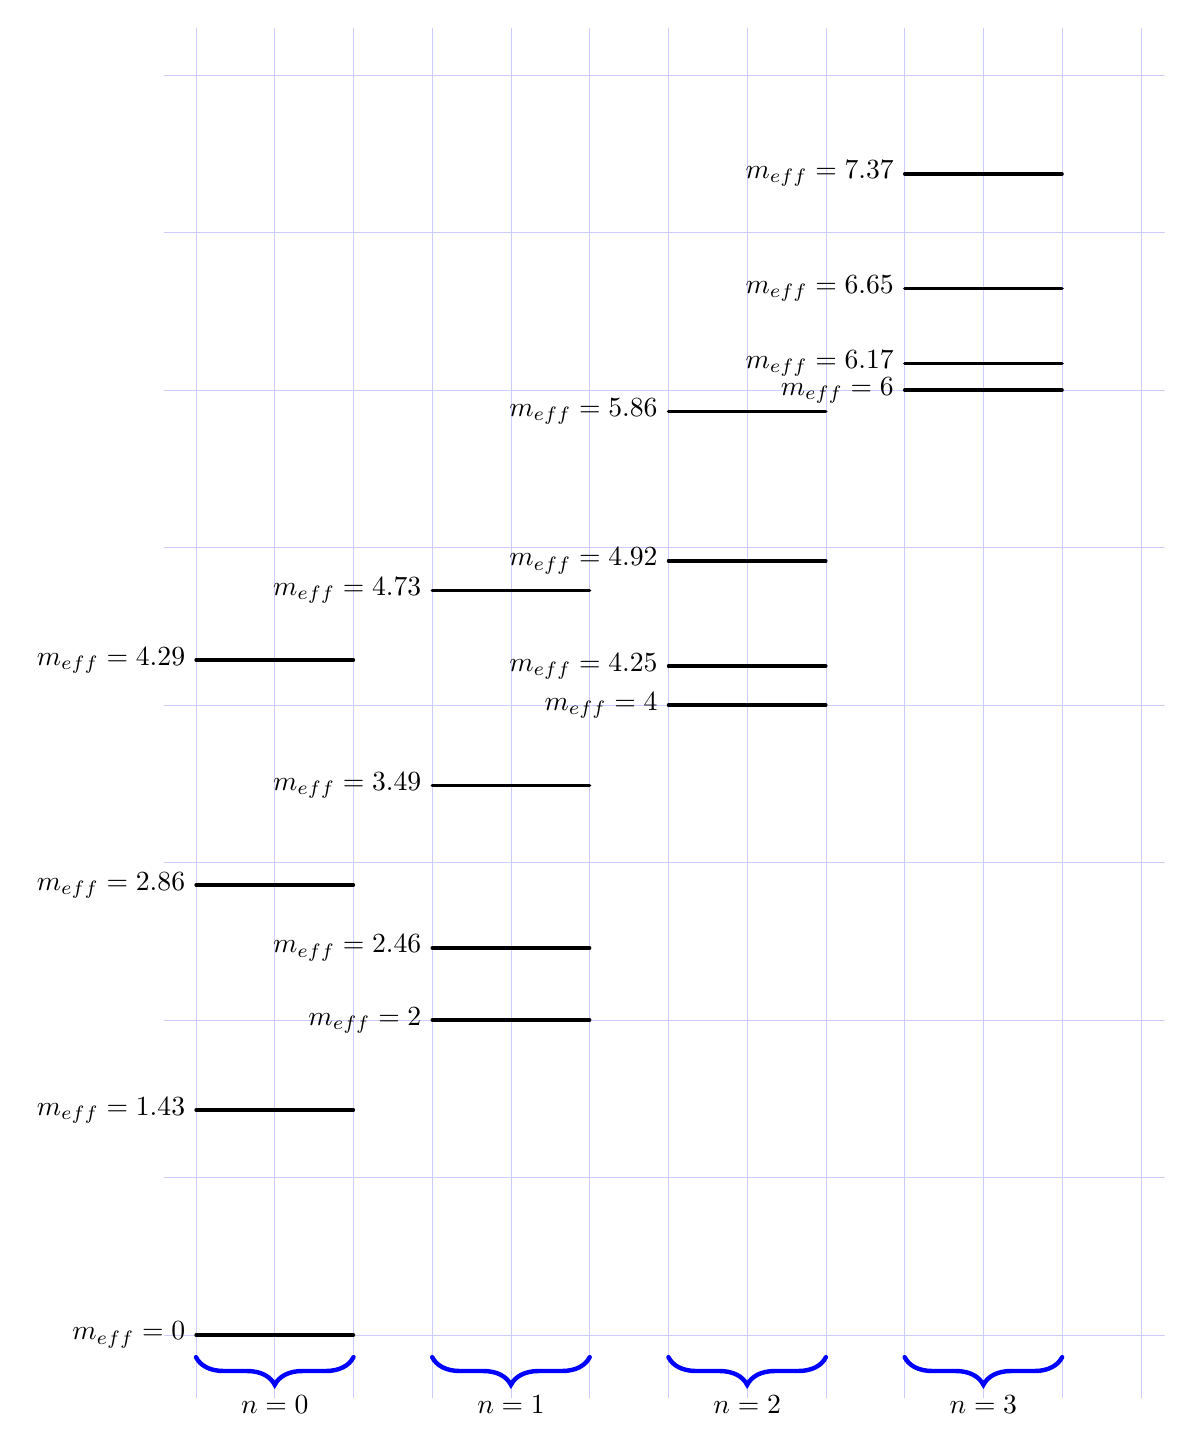
\begin{tikzpicture}[thick,line cap=round,yscale=2,
      % Styles
      axes/.style=,
      important line/.style={very thick},
      information text/.style={rounded corners,draw=blue!80!black,fill=blue!10,inner sep=1ex}]
    \pgfkeys{/pgf/number format/.cd,fixed,precision=2}

    \pgfmathsetmacro{\r}{.7}
    \pgfmathsetmacro{\R}{.5}
    
    \draw[help lines, color=blue!20,step=1cm] (-.4,-.4) grid (12.3,8.3);

    %\draw (0,0) node[anchor=east] {$m_{\text{eff}} =0$} -- (2,0);
    \foreach \n in {0,1,2,3}  {
      \foreach \m in {0,1,...,3} {
        \draw[important line,xshift=3*\n cm] (0,{sqrt((\m/\r)^2 + (\n/\R)^2)}) node[anchor=east] {$m_{\text{eff}} = \pgfmathparse{sqrt((\m/\r)^2 + (\n/\R)^2) }\pgfmathprintnumber{\pgfmathresult}$} -- (2,{sqrt((\m/\r)^2 + (\n/\R)^2)});
      }
      \draw [decorate,decoration={brace,amplitude=10pt,mirror},ultra thick,color=blue,yshift=-4pt,xshift=3*\n cm] (0,0) -- (2,0) node [black,midway,yshift=-0.6cm] { $n=\n$};
    }    
  \end{tikzpicture}
\end{center}


\section{Kaluza-Klein Reduction on $S^1$}

\begin{equation}
  \de{\hat{s}}^2 = e^{2\alpha\phi} \de{s}^2 + e^{2\beta\phi} \left( d\xi + \Ag \right)^2,
\end{equation}

\begin{equation}
  \VIF{a} = 
  \begin{cases}
    \hvif{a} = e^{\alpha\phi} \vif{a}\\
    \hvif{D} = e^{\beta\phi}\left(\df\;\xi +\Ag \right)
  \end{cases},
\end{equation}

From the first Maurer-Cartan equation,
\begin{equation}
  \df\VIF{a} + \SPIF{a}{b}\w\VIF{b} = {\bf{T}}^{\hat{a}} = 0,
\end{equation}
the spin connection can be calculated.
\begin{align}
  \df\hvif{D} =& e^{\beta\phi}\left[\beta\df\;\phi\w\left(\df\;\xi +\Ag \right) + \df\Ag\right]\nonumber\\
  =& e^{\beta\phi}\left[-\beta\left(\df\;\xi +\Ag \right)\w\df\;\phi + \df\Ag\right]\nonumber\\
  =& e^{\beta\phi}\left[-\beta\pa{a}\phi\left(\df\;\xi +\Ag \right)\w\vif{a} + \Fg\right]\nonumber\\
  =& -\beta e^{-\alpha\phi}\pa{a}\phi\;\hvif{D}\w\hvif{a} -\frac{1}{2}e^{(\beta-2\alpha)\phi}\F_{a b}\;\hvif{b}\w\hvif{a},
\end{align}
from where one gets,
\begin{equation}
  \hspif{D}{a} = \beta e^{-\alpha\phi}\pa{a}\phi\hvif{D} + \frac{1}{2}e^{(\beta-2\alpha)\phi}\F_{a b}\hvif{b}.
\end{equation}

On the other hand,
\begin{equation}
  \hspif{a}{b}\w\hvif{b} = -\df\hvif{a} - \hspif{a}{D}\w\hvif{D}.
\end{equation}
Since,
\begin{align}
  \df\hvif{a} 
  =& e^{\alpha\phi}\left[\alpha\df\;\phi\w\vif{a} +  \df\vif{a}\right]\nonumber\\
  =& e^{\alpha\phi}\left[-\alpha\vif{a}\w\df\;\phi -  \spif{a}{b}\w\vif{b}\right]\nonumber\\
  =& -\alpha e^{-\alpha\phi}\pa{b}\phi\;\hvif{a}\w\hvif{b} - \spif{a}{b}\w\hvif{b},
\end{align}
then,
\begin{align}
  \hspif{ab}{} =& \spif{ab}{} + \alpha e^{-\alpha\phi}\pau{b}\phi\hvif{a} - \frac{1}{2}e^{(\beta-2\alpha)\phi}\F^{a b}\hvif{D}\nonumber\\
  =& \spif{ab}{} + \alpha e^{-\alpha\phi}\left(\pau{b}\phi\hvif{a} - \partial^{a}\phi\hvif{b}\right) - \frac{1}{2}e^{(\beta-2\alpha)\phi}\F^{a b}\hvif{D}.
\end{align}

Now, the second Maurer-Cartan equation,
\begin{equation}
  \df\SPIF{a}{b}+\SPIF{a}{c}\w\SPIF{c}{b}=\RIF{a}{b}.
\end{equation}

\begin{align}
  \df\hspif{D a}{} 
  =& \beta\;\df\left( e^{-\alpha\phi}\pau{a}\phi\;\hvif{D}\right) + \frac{1}{2}\df\left(e^{(\beta-2\alpha)\phi}\F^a{}_{b}\;\hvif{b}\right)\nonumber\\
  =& \beta e^{-\alpha\phi}\;\left[-\alpha \pau{a}\phi\;\df\;\phi\w\hvif{D} +\pau{a}\df\;\phi\w\hvif{D} + \pau{a}\phi\;\df\hvif{D}\right]\notag\\
  & + \frac{1}{2}e^{(\beta-2\alpha)\phi}\left[(\beta-2\alpha)\F^a{}_{b}\;\df\;\phi\w\hvif{b} + \df \F^a{}_{b}\w\hvif{b} + \F^a{}_{b}\;\df\hvif{b}\right]\nonumber\\
  =& \beta e^{-\alpha\phi}\;\left[-\alpha \pau{a}\phi\pa{b}\phi\;\vif{b}\w\hvif{D} +\pau{a}\pa{b}\phi\;\vif{b}\w\hvif{D} + \pau{a}\phi\;\hspif{D}{b}\w\hvif{b}\right] \notag\\
  &+ \frac{1}{2}e^{(\beta-2\alpha)\phi}\left[(\beta-2\alpha)\F^a{}_b\pa{c}\phi\;\vif{c}\w\hvif{b} + \pa{c} \F^a{}_b\;\vif{c}\w\hvif{b} + \F^a{}_b\;\hspif{b}{\hat{c}}\w\VIF{c}\right]\nonumber\\
  =& \beta(\beta-\alpha)e^{-2\alpha\phi}\pau{a}\phi\pa{b}\phi\;\hvif{b}\w\hvif{D} + \beta e^{-2\alpha\phi}\pau{a}\pa{b}\phi\;\hvif{b}\w\hvif{D}  \notag\\
  &-\frac{\beta-\alpha}{2}e^{(\beta-3\alpha)\phi}\F^a{}_b\pa{c}\phi\;\hvif{b}\w\hvif{c} +\frac{\beta}{2}e^{(\beta-3\alpha)\phi}\pau{a}\phi \F_{bc}\;\hvif{b}\w\hvif{c}\nonumber\\
  & -\frac{1}{2}e^{(\beta-3\alpha)\phi}\pa{c} \F^a{}_b\;\hvif{b}\w\hvif{c} - \frac{1}{2}e^{(\beta-2\alpha)\phi}\F^a{}_b\; \spif{b}{c}\w\hvif{c},
\end{align}
and,
\begin{align}
  \hspif{D}{m}\w\hspif{m a}{} =& \left(\beta e^{-\alpha\phi}\pa{m}\phi\;\hvif{D} + \frac{1}{2}e^{(\beta-2\alpha)\phi}\F_{m b}\;\hvif{b}  \right)\w\notag\\
  &{}\;\left(\spif{m a}{} + \alpha e^{-\alpha\phi}\left(\pau{a}\phi\;\hvif{m} - \partial^{m}\phi\;\hvif{a}\right) - \frac{1}{2}e^{(\beta-2\alpha)\phi}\F^{m a}\;\hvif{D}  \right)\nonumber\\
  =& \beta e^{-\alpha\phi}\pa{m}\phi\;\hvif{D}\w\spif{m a}{} + \alpha\beta e^{-2\alpha\phi}\pa{m}\phi\;\hvif{D}\w\left(\pau{a}\phi\;\hvif{m} - \partial^{m}\phi\;\hvif{a}\right)\nonumber\\
  & + \frac{1}{2}e^{(\beta-2\alpha)\phi}\F_{m b}\;\hvif{b}\w\spif{m a}{} + \frac{\alpha}{2}e^{(\beta-3\alpha)\phi}\F_{m b}\;\hvif{b}\w\left(\pau{a}\phi\;\hvif{m} - \partial^{m}\phi\;\hvif{a}\right)\nonumber\\
  & -\frac{1}{4}e^{2(\beta-2\alpha)\phi}\F_{m n}\F^{m a}\;\hvif{n}\w\hvif{D}.
\end{align}
Therefore,
\begin{align}
  \hRif{D a}{} =& - \frac{1}{2}e^{(\beta-2\alpha)\phi}\(\F_{bc}\spif{ba}{} + \F^a{}_{b}\; \spif{b}{c}\)\w\hvif{c} + \beta e^{-\alpha\phi}\pa{m}\phi\;\spif{m a}{}\w\hvif{D} \notag\\
  & + \[\beta e^{-2\alpha\phi}\big((\beta-2\alpha)\pa{b}\phi\pau{a}\phi + \pa{b}\pau{a}\phi\big) -\frac{1}{4} e^{2(\beta-2\alpha)\phi}\F_{cb}\F^{ca} \]\hvif{b}\w\hvif{D}\notag\\
  & + \frac{e^{(\beta-3\alpha)\phi}}{2}\bigg[ (\beta-\alpha)\big(\pau{a}\phi\F_{mb} +\pa{m}\phi\F^a{}_b  \big) + \pa{m}\F^a{}_b \bigg] \hvif{m}\w\hvif{b} \notag\\
  & +\alpha\beta e^{-2\alpha\phi}\pa{m}\phi\partial^{m}\phi \;\hvif{a}\w\hvif{D} -\frac{\alpha}{2}e^{(\beta-3\alpha)\phi}\pau{b}\phi\F_{bc}\;\hvif{c}\w\hvif{a}
\end{align}

The second term,
\begin{align}
  \df\hspif{ab}{} =&\quad \df \spif{ab}{} + \df\[\alpha e^{-\alpha\phi}\(\pau{b}\phi\hvif{a}-\pau{a}\phi\hvif{b}\)\]-\frac{1}{2}\df\[e^{(\beta-2\alpha)\phi}\F^{ab}\hvif{D}\]\notag\\
  =&\quad \df \spif{ab}{} + \alpha^2 e^{-2\alpha\phi}\pa{c}\phi\(\pau{b}\phi\hvif{a}-\pau{a}\phi\hvif{b}\)\w\hvif{c}\notag\\
  &\quad -\alpha e^{-2\alpha\phi}\(\pa{c}\pau{b}\phi\hvif{a}-\pa{c}\pau{a}\phi\hvif{b}\)\w\hvif{c}  + \alpha e^{-\alpha\phi}\(\pau{b}\phi\df\hvif{a}-\pau{a}\phi\df\hvif{b}\)\notag\\
  &\quad-\frac{1}{2} e^{(\beta-3\alpha)\phi}\[(\beta-2\alpha)\pa{c}\phi \F^{ab} + \pa{c}\F^{ab}\]\hvif{c}\w\hvif{D}\notag\\
  &\quad  -\frac{1}{2}e^{(\beta-2\alpha)\phi}\F^{ab}\df\hvif{D}\notag\\
  =&\quad \df \spif{ab}{} -\alpha e^{-2\alpha\phi}\(\pa{c}\pau{b}\phi\hvif{a}-\pa{c}\pau{a}\phi\hvif{b}\)\w\hvif{c} \notag\\
  &\quad - \alpha e^{-\alpha\phi}\(\pau{b}\phi\spif{a}{m}-\pau{a}\phi\spif{b}{m}\)\w\hvif{m}-\frac{1}{4} e^{2(\beta-2\alpha)\phi}\F^{ab}\F_{mn}\hvif{m}\w\hvif{n}\\
  &\quad - \frac{1}{2} e^{(\beta-3\alpha)\phi}\[2(\beta-\alpha)\pa{c}\phi \F^{ab} + \pa{c}\F^{ab}\]\hvif{c}\w\hvif{D},\notag%\\
\end{align}
and 
\begin{align}
  \hspif{a}{D}\w\hspif{D b}{} =&\quad -\(  \beta e^{-\alpha\phi}\pau{a}\phi\hvif{D} + \frac{1}{2}e^{(\beta-2\alpha)\phi}\F^{a}{}_m\hvif{m} \)\w\( \beta e^{-\alpha\phi}\pau{b}\phi\hvif{D} + \frac{1}{2}e^{(\beta-2\alpha)\phi}\F^{b}{}_n\hvif{n} \)\notag\\
  =&\quad +\frac{\beta}{2}e^{(\beta-3\alpha)\phi}\(\pau{a}\phi \F^{b}{}_m -\pau{b}\phi\F^{a}{}_m\)\hvif{m}\w\hvif{D}%\notag\\
  %&\quad 
  -  \frac{1}{4}e^{2(\beta-2\alpha)\phi}\F^{a}{}_m \F^{b}{}_n\hvif{m}\w\hvif{n}
\end{align}
\begin{align}
  \hspif{a}{c}\w\hspif{c b}{}  =&\quad \spif{a}{c}\w\spif{c b}{} +\frac{1}{2}e^{(\beta-2\alpha)\phi}\(\F^{a}{}_c \spif{cb}{} -\F^{b}{}_c\spif{ca}{}\)\w\hvif{D}\notag\\
  &\quad +\alpha e^{-\alpha\phi}\( \pau{b}\phi\spif{a}{c}\w\hvif{c} -\pau{c}\phi\spif{a}{c}\w\hvif{b} + \pau{c}\phi\spif{b}{c}\w\hvif{a} - \pau{a}\phi\spif{b}{c}\w\hvif{c}  \) \notag\\
  &\quad +\alpha^2 e^{-2\alpha\phi}\( \pau{b}\phi\pa{c}\phi\hvif{a}\w\hvif{c} -\pau{a}\phi\pa{c}\phi\hvif{b}\w\hvif{c} - \pau{c}\phi\pa{c}\phi\hvif{a}\w\hvif{b}  \) \notag\\
  &\quad +\frac{\alpha}{2}e^{(\beta-3\alpha)\phi}\[\F^b{}_c\(\pau{c}\phi\hvif{a} - \pau{a}\phi\hvif{c}\)  + \F^a{}_c\(\pau{b}\phi\hvif{c} - \pau{c}\phi\hvif{b}\)   \]\w\hvif{D}.
\end{align}

Next, one can write the Lagrangian of the higher dimensional spacetime,
\begin{align}
  \Lag_{(D+1)} =& \frac{\epsilon_{\hat{a}_1\hat{a}_2\cdots\hat{a}_{D+1}}}{(D-1)!}\hRif{\hat{a}_1\hat{a}_2}{}\w\hvif{\hat{a}_3}\w\cdots\w\hvif{\hat{a}_{D+1}}\\
  =& \underbrace{2\frac{\epsilon_{D a_1 a_2\cdots a_{D}}}{(D-1)!}\hRif{D{a}_1}{}\w\hvif{{a}_2}\w\cdots\w\hvif{{a}_{D}}}_{\text{Term }I}\notag\\
  &+ \underbrace{\frac{\epsilon_{a_1 a_2\cdots a_{D}D}}{(D-2)!}\hRif{{a}_1{a}_2}{}\w\hvif{{a}_3}\w\cdots\w\hvif{{a}_{D}}\w\hvif{D}}_{\text{Term }II}.
\end{align}
Concentrate on the first term,
\begin{align}
  I =&\quad 2(-1)^D \frac{\epsilon_{a_1 a_2\cdots a_{D}}}{(D-1)!}\notag\\
  &\qquad\bigg\{\[\beta e^{-2\alpha\phi}\big((\beta-2\alpha)\pa{b}\phi\pau{a_1}\phi + \pa{b}\pau{a_1}\phi\big) -\frac{1}{4} e^{2(\beta-2\alpha)\phi}\F_{cb}\F^{ca_1} \]\hvif{b}\notag\\
  &\qquad + \beta e^{-\alpha\phi}\pa{m}\phi\;\spif{m a_1}{}+\alpha\beta e^{-2\alpha\phi}\pa{m}\phi\partial^{m}\phi \;\hvif{a}\bigg\}\w\hvif{D}\w\hvif{{a}_2}\w\cdots\w\hvif{{a}_{D}}\notag\\
  =&\quad -2\frac{\epsilon_{a_1 a_2\cdots a_{D}}}{(D-1)!}\notag\\
  &\qquad\bigg\{\[\beta e^{-2\alpha\phi}\big((\beta-2\alpha)\pa{b}\phi\pau{a_1}\phi + \pa{b}\pau{a_1}\phi\big) -\frac{1}{4} e^{2(\beta-2\alpha)\phi}\F_{cb}\F^{ca_1} \]\hvif{b}\notag\\
  &\qquad + \beta e^{-\alpha\phi}\pa{m}\phi\;\spif{m a_1}{}+\alpha\beta e^{-2\alpha\phi}\pa{m}\phi\partial^{m}\phi \;\hvif{a}\bigg\}\w\hvif{{a}_2}\w\cdots\w\hvif{{a}_{D}}\w\hvif{D}\notag\\
  =&\quad -2\frac{\epsilon_{a_1 a_2\cdots a_{D}}}{(D-1)!} e^{\((D-2)\alpha+\beta\)\phi}\notag\\
  &\qquad\bigg\{\[\beta \big((\beta-2\alpha)\pa{b}\phi\pau{a_1}\phi + \pa{b}\pau{a_1}\phi\big) -\frac{1}{4} e^{2(\beta-\alpha)\phi}\F_{cb}\F^{ca_1} \]\vif{b}\notag\\
  &\qquad + \beta \pa{m}\phi\;\(\spi{b}\)^{m a_1}\vif{b}+\alpha\beta \pa{m}\phi\partial^{m}\phi \;\vif{a_1}\bigg\}\w\vif{{a}_2}\w\cdots\w\vif{{a}_{D}}\w\df\;\xi\notag\\
  =&\quad -2 e^{\((D-2)\alpha+\beta\)\phi}\bigg\{\beta \big((\beta-2\alpha)\pa{b}\phi\pau{b}\phi + \pa{b}\pau{b}\phi\big)
  %% \notag\\
  %% &\qquad
  -\frac{1}{4} e^{2(\beta-\alpha)\phi}\F_{cb}\F^{cb} \notag\\
  &\qquad\quad + \beta \pa{m}\phi\;\(\spi{b}\)^{m b} + D \alpha\beta \;\pa{m}\phi\partial^{m}\phi \bigg\}\de{V_D}\de{\xi}
\end{align}

\begin{align}
  II =&\quad \frac{\epsilon_{a_1 a_2\cdots a_{D}D}}{(D-2)!}\notag\\
  &\qquad \bigg\{\Rif{a_1a_2}{} -\alpha e^{-2\alpha\phi}\(\pa{c}\pau{a_2}\phi\hvif{a_1}-\pa{c}\pau{a_1}\phi\hvif{a_2}\)\w\hvif{c}\notag\\
  &\qquad -\frac{1}{4} e^{2(\beta-2\alpha)\phi}\(\F^{a_1a_2}\F_{mn}+\F^{a_1}{}_m \F^{a_2}{}_n\)\hvif{m}\w\hvif{n}\notag\\
  &\qquad +\alpha e^{-\alpha\phi}\( \pau{a_2}\phi\spif{a_1}{c}\w\hvif{c} -\pau{c}\phi\spif{a_1}{c}\w\hvif{a_2} + \pau{c}\phi\spif{a_2}{c}\w\hvif{a_1} - \pau{a_1}\phi\spif{a_2}{c}\w\hvif{c}  \) \notag\\
  &\qquad +\alpha^2 e^{-2\alpha\phi}\( \pau{a_2}\phi\pa{c}\phi\hvif{a_1}\w\hvif{c} -\pau{a_1}\phi\pa{c}\phi\hvif{a_2}\w\hvif{c} - \pau{c}\phi\pa{c}\phi\hvif{a_1}\w\hvif{a_2}  \) \notag\\
  &\qquad - \alpha e^{-\alpha\phi}\(\pau{a_2}\phi\spif{a_1}{m}-\pau{a_1}\phi\spif{a_2}{m}\)\w\hvif{m}\bigg\}\w\hvif{{a}_3}\w\cdots\w\hvif{{a}_{D}}\w\hvif{D}\notag\\
  =&\quad \frac{\epsilon_{a_1 a_2\cdots a_{D}}}{(D-2)!}e^{\((D-2)\alpha+\beta\)\phi}\notag\\
  &\qquad \bigg\{\Rif{a_1a_2}{} -\alpha \(\pa{c}\pau{a_2}\phi\vif{a_1}-\pa{c}\pau{a_1}\phi\vif{a_2}\)\w\vif{c}\notag\\
  &\qquad -\frac{1}{4} e^{2(\beta-\alpha)\phi}\(\F^{a_1a_2}\F_{mn}+\F^{a_1}{}_m \F^{a_2}{}_n\)\vif{m}\w\vif{n}\notag\\
  &\qquad +\alpha \( \pau{a_2}\phi\spif{a_1}{n}\w\vif{n} -\pau{c}\phi\spif{a_1}{c}\w\vif{a_2} + \pau{c}\phi\spif{a_2}{c}\w\vif{a_1} - \pau{a_1}\phi\spif{a_2}{n}\w\vif{n}  \) \notag\\
  &\qquad +\alpha^2 \( \pau{a_2}\phi\pa{c}\phi\vif{a_1}\w\vif{c} -\pau{a_1}\phi\pa{c}\phi\vif{a_2}\w\vif{c} - \pau{c}\phi\pa{c}\phi\vif{a_1}\w\vif{a_2}  \) \notag\\
  &\qquad - \alpha \(\pau{a_2}\phi\spif{a_1}{n}-\pau{a_1}\phi\spif{a_2}{n}\)\w\vif{n}\bigg\}\w\vif{{a}_3}\w\cdots\w\vif{{a}_{D}}\w\df\;\xi\notag\\
  =&\quad \frac{\epsilon_{a_1 a_2\cdots a_{D}}}{(D-2)!}e^{\((D-2)\alpha+\beta\)\phi} \notag\\
  &\qquad \bigg\{\Rif{a_1a_2}{}  - \alpha^2 \pau{c}\phi\pa{c}\phi\vif{a_1}\w\vif{a_2} \notag\\
  &\qquad  -\frac{1}{4} e^{2(\beta-\alpha)\phi}\(\F^{a_1a_2}\F_{mn}+\F^{a_1}{}_m \F^{a_2}{}_n\)\vif{m}\w\vif{n}\notag\\
  &\qquad +\alpha \[\alpha \pau{a_2}\phi\pa{c}\phi - \pa{c}\pau{a_2}\phi - \pau{m}\phi\(\spi{c}\)^{a_2}{}_{m}  \]\vif{a_1}\w\vif{c} \notag\\
  &\qquad -\alpha \[\alpha \pau{a_1}\phi\pa{c}\phi - \pa{c}\pau{a_1}\phi - \pau{m}\phi\(\spi{c}\)^{a_1}{}_{m}  \]\vif{a_2}\w\vif{c} \bigg\}\w\vif{{a}_3}\w\cdots\w\vif{{a}_{D}}\w\df\;\xi\notag\\
  =&\quad e^{\((D-2)\alpha+\beta\)\phi}\de{V_D}\de{\xi}\bigg\{\Ri - D(D-1)\alpha^2 \pau{c}\phi\pa{c}\phi - \frac{1}{4} e^{2(\beta-\alpha)\phi}\F_{mn}\F^{mn}\notag\\
  &\qquad + 2(D-1)\alpha \big[\alpha \pau{c}\phi\pa{c}\phi - \pa{c}\pau{c}\phi - \pau{m}\phi\(\spi{c}\)^{c}{}_{m}  \big]\bigg\}
\end{align}

Therefore,
\begin{align}
  \Lag_{(D+1)} =&\quad  e^{\((D-2)\alpha+\beta\)\phi}\de{V_D}\de{\xi}\bigg\{\Ri - D(D-1)\alpha^2 \pau{c}\phi\pa{c}\phi - \frac{1}{4} e^{2(\beta-\alpha)\phi}\F_{mn}\F^{mn}\notag\\
  &\qquad + 2(D-1)\alpha \big[\alpha \pau{c}\phi\pa{c}\phi - \pa{c}\pau{c}\phi - \pau{m}\phi\(\spi{c}\)^{c}{}_{m}  \big]\notag\\
  &\qquad -2\beta \big((\beta-2\alpha)\pa{b}\phi\pau{b}\phi + \pa{b}\pau{b}\phi\big) +\frac{1}{2} e^{2(\beta-\alpha)\phi}\F_{cb}\F^{cb} \notag\\
  &\qquad -2 \beta \pa{m}\phi\;\(\spi{b}\)^{m b} -2 D \alpha\beta \;\pa{m}\phi\partial^{m}\phi \bigg\}\notag\\
  =&\quad  e^{\((D-2)\alpha+\beta\)\phi}\de{V_D}\de{\xi}\bigg\{\Ri - \[(D-1)(D-2)\alpha^2 +2\beta(\beta-2\alpha) + 2D\alpha\beta\]\pau{c}\phi\pa{c}\phi\notag\\
  &\qquad + \frac{1}{4} e^{2(\beta-\alpha)\phi}\F_{mn}\F^{mn} - 2\[(D-1)\alpha +\beta\]\Box\phi - 2\[(D-1)\alpha -\beta\]\pa{m}\phi\(\spi{c}\)^{cm}\bigg\}
\end{align}

One can choose $\beta=-(D-2)\alpha$, so that the result on the compactification would give $D$-dimensional gravity on the ``Einstein'' frame, then
\begin{align}
  \Lag_{(D+1)} =&\quad  \de{V_D}\de{\xi}\bigg\{\Ri - (D-1)(D-2)\alpha^2\pau{c}\phi\pa{c}\phi\notag\\
  &\qquad + \frac{1}{4} e^{-2(D-1)\alpha\phi}\F_{mn}\F^{mn} \bigg\},%- 2\[(D-1)\alpha +\beta\]\Box\phi - 2\[(D-1)\alpha -\beta\]\pa{m}\phi\(\spi{c}\)^{cm}\bigg\}
\end{align}
where the other terms were dropped because are a boundary term. Additionally, in order to get the usual kinetic term for the scalar field, i.e., 
\begin{equation}
  \alpha^2 = \frac{1}{2}\frac{1}{(D-1)(D-2)},
\end{equation}
finally
\begin{equation}
  \Lag_{(D+1)} =\;  \de{V_D}\de{\xi}\bigg\{\Ri - \frac{1}{2}\pau{c}\phi\pa{c}\phi + \frac{1}{4} e^{-2(D-1)\alpha\phi}\F_{mn}\F^{mn} \bigg\}.
\end{equation}
